\chapter{Grundlagen}
Dieses Kapitel befasst sich mit sowohl den mathematischen als auch den technischen Grundlagen der zu behandelnden Thematik, welche für das weitere Verständnis der Arbeit beitragen. \textit{Auf mobile Anwendungen geht dieses Grundlagenkapitel nicht in besonderer Tiefe ein, da ein allgemeines Verständnis und Vertrautheit mit Konzepten und Technologien mobiler Anwendungen vorausgesetzt wird.}
\section{Mathematische Grundlagen}
\subsection*{Berechnung der Geschwindigkeitsempfehlung}
Präsentiert das System während der Anwendung eine Geschwindigkeitsempfehlung, ist diese abhängig von der Fahrtgeschwindigkeit und vom Abstand zur Ampel. Angenommen die Progressionsgeschwindigkeit $V$ wird zum Zeitpunkt $t_{1}$ ausgesprochen, die \gls {LSA} schaltet zum Zeitpunt $t_{2}$ auf Rot und Abstand zur Ampel beträgt $S$, dann gilt: 
\[ V = \frac{S}{t_{2} - t_{1}} \]
Um die ensprechende \gls{LSA} während der Grünphase zu passieren, muss letztendlich die empfohlene Geschwindigkeit $V$ eingehalten werden. Folgende Fälle werden beachtet:
\paragraph{Anhalten ist unvermeidbar:} Die Ampelschaltung erlaubt momentan kein reibungsloses Passieren. 
\textit{Umgesetzte Anzeigevariante: \textbf{rot}}
\paragraph{Konstante Weiterfahrt möglich:} Ist die empfohlene Geschwindigkeit gleich der aktuellen, ist ein reibungsloses Passieren bei beibehaltenem Tempo möglich. Es besteht kein Handlungsbedarf. 
\textit{Umgesetzte Anzeigevariante: \textbf{grün}}
\paragraph{Reibungsloses Passieren durch Beschleunigung möglich:} Zeigt die Ampel im Moment Grün und ist die empfohlene Geschwindigkeit höher als die aktuelle, ist ein reibungsloses Passieren durch Beschleunigung zu erreichen. Bei der Anzeige der Progressionsgeschwindigkeit ist selbstverständlich die geltende Höchstgeschwindigkeitsbegrenzung zu beachten. 
\textit{Umgesetzte Anzeigevariante: \textbf{grün}}
\paragraph{Reibungsloses Passieren duch Verlangsamen möglich:} Zeigt die Ampel im Moment Rot und ist die empfohlene Geschwindigkeit niedriger als die aktuelle, ist ein reibungsloses Passieren durch Verlangsamung zu erreichen.
\textit{Umgesetzte Anzeigevariante: \textbf{grün}}
%\subsection{Berechnung der Restrotanzeige}
% ist aber trivial
% -------------------------------------------------
% TECHNISCHE GRUNDLAGEN
% -------------------------------------------------
\section{Technische Grundlagen}
Im folgenden Abschnitt werden Funktionsweise und Besonderheiten der verwendeten Technologien beschrieben.
% ANGULAR
\subsection{Hybride App mit AngularJS + Phonegap?}
% JavaScript
\subsection{JavaScript?}
% NODEJS
\subsection{\label{Node.js}Node.js}
Node.js ist ein Framework zur Entwicklung serverseitiger Netzwerkanwendungen und basiert auf dem JavaScript Interpreter V8 des Chrome Browsers -- verfügt daher über eine überaus hohe Performance. Darüber hinaus können durch die fundamentalen Konzepte Streaming und Websockets\footnote{ Websockets dienen beispielsweise Anwendungen, bei denen der Webserver dem Client auch nach abgeschlossener Übertragung der Webseite Push-Nachrichten senden kann.} echtzeitfähige Webanwendungen entwickelt werden\footnote{ Vgl. \cite{nodeCo} S. 7}. \\\\
Eine Besonderheit stellt die Handhabung von Threads in Node.js dar:
Anders als bei klassische Webservern, deren Threads die meiste Zeit mit Warten auf die Beendigung einer I/O-Operation beschäftigt sind, verwendet Node.js hierfür eine interne Threadimplementierung, die sogenannte Event-Loop. 
\begin{figure}[H]
 \centering
    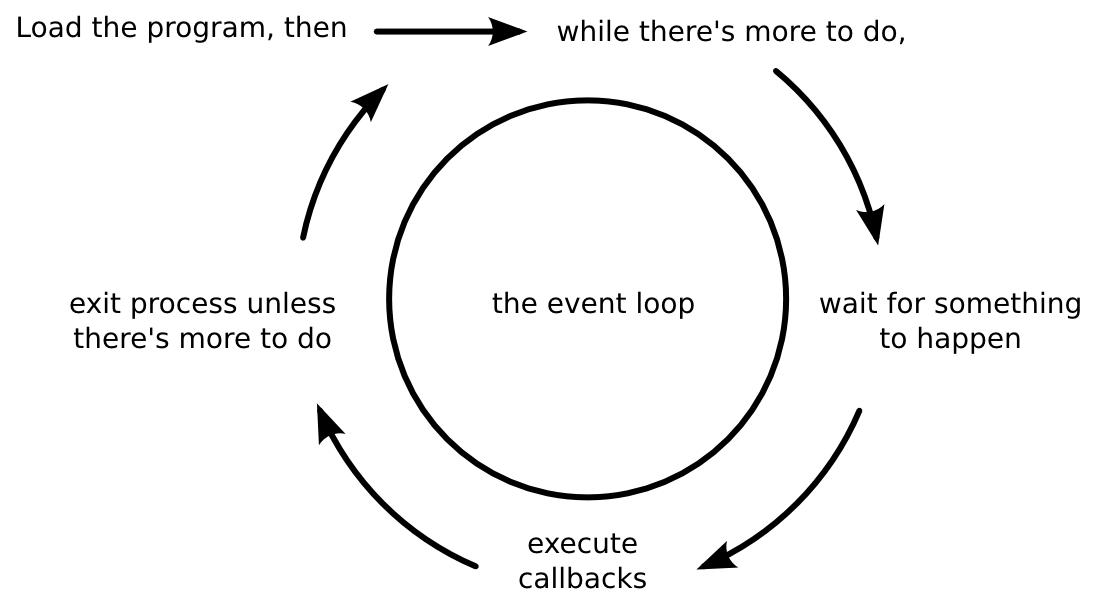
\includegraphics[width=0.7\textwidth]{eventloop}
\caption[Node.js Event-Loop]{Node.js Event-Loop Quelle: \cite{nodeWay} S. 3}
\label{fig:Nodejs_eventloop}
\end{figure}
Der Begriff "'Event-Loop"' in Node.js impliziert die asynchrone Ausführung von unter anderem I/O-Operationen, die Verwaltung der Callback-Funktionen, welche beim Aufruf dieser Operationen übergeben werden und den Aufruf einer Callback-Funktion, sobald das Ergebnis der Operation vorliegt\footnote{ Vgl. \cite{nodeCo} S. 11f}.
\begin{quote}
"' Node simply enters the event loop after executing the input script. Node exits the event loop when there are no more callbacks to perform."' (\cite{node})
\end{quote}
Um die Fähigkeiten von Node.js zu steigern, können Module ergänzt werden. Einige, wie zum Beispiel das \textit{http}-Modul in dem Funktionen zur Implementierung von Webservern enthalten sind, sind bereits in der Standardinstallation enthalten. 
Eine weitere Eigenschaft ist der Einsatz sogenannter \textit{Middlewares}. Diese dienen der Kapselung von eingehenden Requests und der verarbeitenden Webanwendung. So durchläuft die Anfrage erst jedes einzelne Modul\footnote{ zum Beispiel Internationalisierung und Authentifizierung} der Middleware bevor sie die Webanwendung erreicht\footnote{ Vgl. \cite{nodeCo} S. 145ff}. Unter dem Einsatz von Middlewares und anderer Bestandteile lassen sich mit wenig Aufwand \gls{RESTg}-\glspl{API} entwerfen.
% MONGODB NOSQL
\subsection{NoSQL Datenbank MongoDB}
Eine inzwischen weit verbreitete Alternative zu \gls{SQL} Datenbanken sind die \gls{NoSQL} Datenbanken. MongoDB\footnote{ Namensherkunft: hu\textbf{mongo}us, dt.: 'riesig', 'enorm', 'gigantisch'} ist eine dokumentenorientierte Open Sourche Datenbanktechnologie und eigener Aussage zufolge derzeit "'the leading NoSQL Database..."' (\cite{mongodb}). \\
Eine dokumentenorientierte \gls{NoSQL}-Datenbank übernimmt beispielsweise die Daten, die gespeichert werden sollen und aggregiert sie in Dokumente im \gls{JSON}-Format, welches wiederum als Objekt betrachtet werden kann. Dieser Ansatz ermöglicht es in einem einzigen Datensatz komplexe hierarchische Beziehungen darzustellen. Dadurch können die Dokumente effizienter und einfacher verteilt werden und der Lese-und Schreibzugriff wird performanter. Während also relationale Datenbanksysteme auf Tabellen aufbauen, basiert MongoDB auf sogenannten Collections, einer Menge von Dokumenten\footnote{ Vgl. \cite{mongoDef} S. 7}. Das Datenformat für Dokumente in MongoDB ist BSON (Binaray JSON), eine Erweiterung von \gls{JSON} um einige binäre Typen. Zu den unterstützten Datentypen gehören also neben \textit{Strings}, \textit{Numbers}, \textit{Objects}, \textit{Arrays}, \textit{Null}, \textit{Boolean} auch \textit{Date} Objekte, \textit{Reguläre Ausdrücke}, \textit{ObjectIDs} und \textit{eingebettete Dokumente}\footnote{ Vgl. \cite{mongoDef} S. 17ff}. Ein Dokument könnte demnach so aussehen: \\
\lstinputlisting
	[caption={Ein MongoDB Dokument}
	\label{code:mongo}, captionpos=b, language=XML]{code/mongoDoc.js}
In relationalen Datenbanken haben Entitäten ein striktes Schema, was bedeutet dass alle Reihen einer Tabelle die selben Spalten besitzen muss. In MongoDB gibt es keine vordefinierten Schemata: Schlüssel und Werte eines Dokuments sind nicht von festen Typen oder Größen. Ohne festes Schema ist das Hinzufügen oder Entfernen von Feldern jederzeit möglich ohne die Anwendung zu beeinträchtigen.\\
\textbf{\large TODO: mongoose auch?}
stellt einen objektrelationalen Mapper einschließlich einer anpass und erweiterbaren middleware zur verfügung
\subsubsection*{Mobile Sensing?}
